% GNUPLOT: LaTeX picture with Postscript
\begingroup
  \makeatletter
  \providecommand\color[2][]{%
    \GenericError{(gnuplot) \space\space\space\@spaces}{%
      Package color not loaded in conjunction with
      terminal option `colourtext'%
    }{See the gnuplot documentation for explanation.%
    }{Either use 'blacktext' in gnuplot or load the package
      color.sty in LaTeX.}%
    \renewcommand\color[2][]{}%
  }%
  \providecommand\includegraphics[2][]{%
    \GenericError{(gnuplot) \space\space\space\@spaces}{%
      Package graphicx or graphics not loaded%
    }{See the gnuplot documentation for explanation.%
    }{The gnuplot epslatex terminal needs graphicx.sty or graphics.sty.}%
    \renewcommand\includegraphics[2][]{}%
  }%
  \providecommand\rotatebox[2]{#2}%
  \@ifundefined{ifGPcolor}{%
    \newif\ifGPcolor
    \GPcolortrue
  }{}%
  \@ifundefined{ifGPblacktext}{%
    \newif\ifGPblacktext
    \GPblacktexttrue
  }{}%
  % define a \g@addto@macro without @ in the name:
  \let\gplgaddtomacro\g@addto@macro
  % define empty templates for all commands taking text:
  \gdef\gplbacktext{}%
  \gdef\gplfronttext{}%
  \makeatother
  \ifGPblacktext
    % no textcolor at all
    \def\colorrgb#1{}%
    \def\colorgray#1{}%
  \else
    % gray or color?
    \ifGPcolor
      \def\colorrgb#1{\color[rgb]{#1}}%
      \def\colorgray#1{\color[gray]{#1}}%
      \expandafter\def\csname LTw\endcsname{\color{white}}%
      \expandafter\def\csname LTb\endcsname{\color{black}}%
      \expandafter\def\csname LTa\endcsname{\color{black}}%
      \expandafter\def\csname LT0\endcsname{\color[rgb]{1,0,0}}%
      \expandafter\def\csname LT1\endcsname{\color[rgb]{0,1,0}}%
      \expandafter\def\csname LT2\endcsname{\color[rgb]{0,0,1}}%
      \expandafter\def\csname LT3\endcsname{\color[rgb]{1,0,1}}%
      \expandafter\def\csname LT4\endcsname{\color[rgb]{0,1,1}}%
      \expandafter\def\csname LT5\endcsname{\color[rgb]{1,1,0}}%
      \expandafter\def\csname LT6\endcsname{\color[rgb]{0,0,0}}%
      \expandafter\def\csname LT7\endcsname{\color[rgb]{1,0.3,0}}%
      \expandafter\def\csname LT8\endcsname{\color[rgb]{0.5,0.5,0.5}}%
    \else
      % gray
      \def\colorrgb#1{\color{black}}%
      \def\colorgray#1{\color[gray]{#1}}%
      \expandafter\def\csname LTw\endcsname{\color{white}}%
      \expandafter\def\csname LTb\endcsname{\color{black}}%
      \expandafter\def\csname LTa\endcsname{\color{black}}%
      \expandafter\def\csname LT0\endcsname{\color{black}}%
      \expandafter\def\csname LT1\endcsname{\color{black}}%
      \expandafter\def\csname LT2\endcsname{\color{black}}%
      \expandafter\def\csname LT3\endcsname{\color{black}}%
      \expandafter\def\csname LT4\endcsname{\color{black}}%
      \expandafter\def\csname LT5\endcsname{\color{black}}%
      \expandafter\def\csname LT6\endcsname{\color{black}}%
      \expandafter\def\csname LT7\endcsname{\color{black}}%
      \expandafter\def\csname LT8\endcsname{\color{black}}%
    \fi
  \fi
  \setlength{\unitlength}{0.0500bp}%
  \begin{picture}(7200.00,5040.00)%
    \gplgaddtomacro\gplbacktext{%
      \csname LTb\endcsname%
      \put(948,3066){\makebox(0,0)[r]{\strut{}-1}}%
      \csname LTb\endcsname%
      \put(948,3360){\makebox(0,0)[r]{\strut{}-0.5}}%
      \csname LTb\endcsname%
      \put(948,3654){\makebox(0,0)[r]{\strut{}0}}%
      \csname LTb\endcsname%
      \put(948,3947){\makebox(0,0)[r]{\strut{}0.5}}%
      \csname LTb\endcsname%
      \put(948,4241){\makebox(0,0)[r]{\strut{}1}}%
      \csname LTb\endcsname%
      \put(1080,2552){\makebox(0,0){\strut{}}}%
      \csname LTb\endcsname%
      \put(1656,2552){\makebox(0,0){\strut{}}}%
      \csname LTb\endcsname%
      \put(2232,2552){\makebox(0,0){\strut{}}}%
      \csname LTb\endcsname%
      \put(2807,2552){\makebox(0,0){\strut{}}}%
      \csname LTb\endcsname%
      \put(3383,2552){\makebox(0,0){\strut{}}}%
      \put(178,3653){\rotatebox{-270}{\makebox(0,0){\strut{}$\varphi/\varphi_0$}}}%
    }%
    \gplgaddtomacro\gplfronttext{%
      \csname LTb\endcsname%
      \put(2972,4362){\makebox(0,0)[r]{\strut{}Dämpfung 0mm}}%
    }%
    \gplgaddtomacro\gplbacktext{%
      \csname LTb\endcsname%
      \put(3828,3066){\makebox(0,0)[r]{\strut{}}}%
      \csname LTb\endcsname%
      \put(3828,3360){\makebox(0,0)[r]{\strut{}}}%
      \csname LTb\endcsname%
      \put(3828,3654){\makebox(0,0)[r]{\strut{}}}%
      \csname LTb\endcsname%
      \put(3828,3947){\makebox(0,0)[r]{\strut{}}}%
      \csname LTb\endcsname%
      \put(3828,4241){\makebox(0,0)[r]{\strut{}}}%
      \csname LTb\endcsname%
      \put(3960,2552){\makebox(0,0){\strut{}}}%
      \csname LTb\endcsname%
      \put(4536,2552){\makebox(0,0){\strut{}}}%
      \csname LTb\endcsname%
      \put(5112,2552){\makebox(0,0){\strut{}}}%
      \csname LTb\endcsname%
      \put(5687,2552){\makebox(0,0){\strut{}}}%
      \csname LTb\endcsname%
      \put(6263,2552){\makebox(0,0){\strut{}}}%
    }%
    \gplgaddtomacro\gplfronttext{%
      \csname LTb\endcsname%
      \put(5852,4362){\makebox(0,0)[r]{\strut{}Dämpfung 4mm}}%
    }%
    \gplgaddtomacro\gplbacktext{%
      \csname LTb\endcsname%
      \put(948,1302){\makebox(0,0)[r]{\strut{}-1}}%
      \csname LTb\endcsname%
      \put(948,1596){\makebox(0,0)[r]{\strut{}-0.5}}%
      \csname LTb\endcsname%
      \put(948,1890){\makebox(0,0)[r]{\strut{}0}}%
      \csname LTb\endcsname%
      \put(948,2183){\makebox(0,0)[r]{\strut{}0.5}}%
      \csname LTb\endcsname%
      \put(948,2477){\makebox(0,0)[r]{\strut{}1}}%
      \csname LTb\endcsname%
      \put(1080,788){\makebox(0,0){\strut{}0}}%
      \csname LTb\endcsname%
      \put(1656,788){\makebox(0,0){\strut{}5}}%
      \csname LTb\endcsname%
      \put(2232,788){\makebox(0,0){\strut{}10}}%
      \csname LTb\endcsname%
      \put(2807,788){\makebox(0,0){\strut{}15}}%
      \csname LTb\endcsname%
      \put(3383,788){\makebox(0,0){\strut{}20}}%
      \put(178,1889){\rotatebox{-270}{\makebox(0,0){\strut{}$\varphi/\varphi_0$}}}%
      \put(2519,458){\makebox(0,0){\strut{}$t [s]$}}%
    }%
    \gplgaddtomacro\gplfronttext{%
      \csname LTb\endcsname%
      \put(2972,2598){\makebox(0,0)[r]{\strut{}Dämpfung 6mm}}%
    }%
    \gplgaddtomacro\gplbacktext{%
      \csname LTb\endcsname%
      \put(3828,1302){\makebox(0,0)[r]{\strut{}}}%
      \csname LTb\endcsname%
      \put(3828,1596){\makebox(0,0)[r]{\strut{}}}%
      \csname LTb\endcsname%
      \put(3828,1890){\makebox(0,0)[r]{\strut{}}}%
      \csname LTb\endcsname%
      \put(3828,2183){\makebox(0,0)[r]{\strut{}}}%
      \csname LTb\endcsname%
      \put(3828,2477){\makebox(0,0)[r]{\strut{}}}%
      \csname LTb\endcsname%
      \put(3960,788){\makebox(0,0){\strut{}0}}%
      \csname LTb\endcsname%
      \put(4536,788){\makebox(0,0){\strut{}5}}%
      \csname LTb\endcsname%
      \put(5112,788){\makebox(0,0){\strut{}10}}%
      \csname LTb\endcsname%
      \put(5687,788){\makebox(0,0){\strut{}15}}%
      \csname LTb\endcsname%
      \put(6263,788){\makebox(0,0){\strut{}20}}%
      \put(5399,458){\makebox(0,0){\strut{}$t [s]$}}%
    }%
    \gplgaddtomacro\gplfronttext{%
      \csname LTb\endcsname%
      \put(5852,2598){\makebox(0,0)[r]{\strut{}Dämpfung 8mm}}%
    }%
    \gplbacktext
    \put(0,0){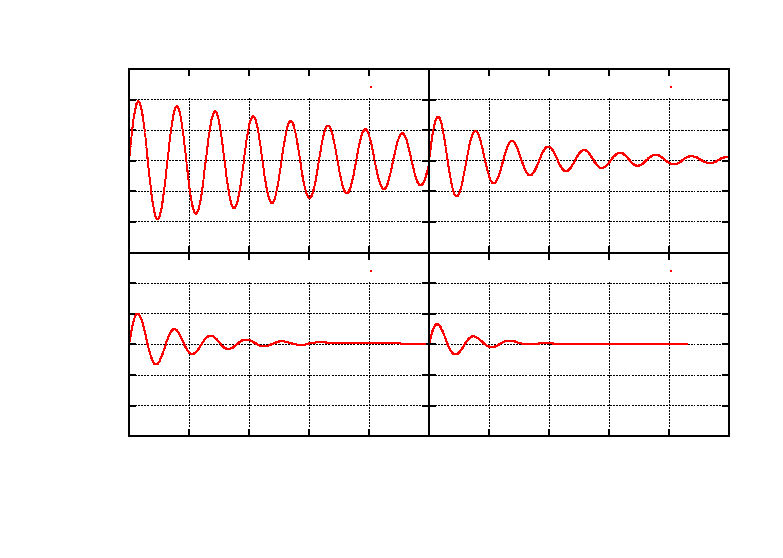
\includegraphics{plot_dif0}}%
    \gplfronttext
  \end{picture}%
\endgroup
